\chapter{Grundlagen}
\label{chap:grundlagen}
Container werden häufig als leichtgewichtige \glspl{acr-vm} beschrieben. Dies ist allerdings nicht ganz richtig. Wie in \fref{fig:containerVsVm} zu erkennen, virtualisieren Container kein vollständiges \gls{acr-os}, sondern lediglich das benötigte Dateisystem. Dabei wird der \gls{gls-kernel} des Hosts nicht virtualisiert, sondern mitverwendet. Dies macht Container deutlich leichtgewichtiger als \glspl{acr-vm}, isoliert allerdings weniger umfangreich als diese. So werden bei Containern \gls{gls-kernel}funktionen mit dem Host-\gls{acr-os} geteilt. \glspl{acr-vm} isolieren diese Funktionen in eigenen virtuellen Betriebssystemen.
\begin{figure}[h]
		\subfigure[Container]{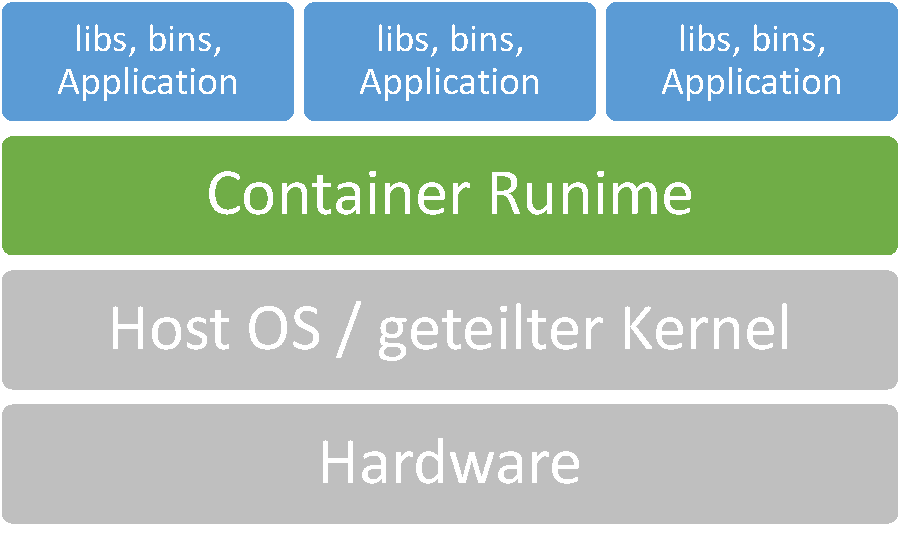
\includegraphics[width=0.49\textwidth]{bilder/container-stack-isolation.pdf}}
		\hfill
		\subfigure[\glspl{acr-vm}]{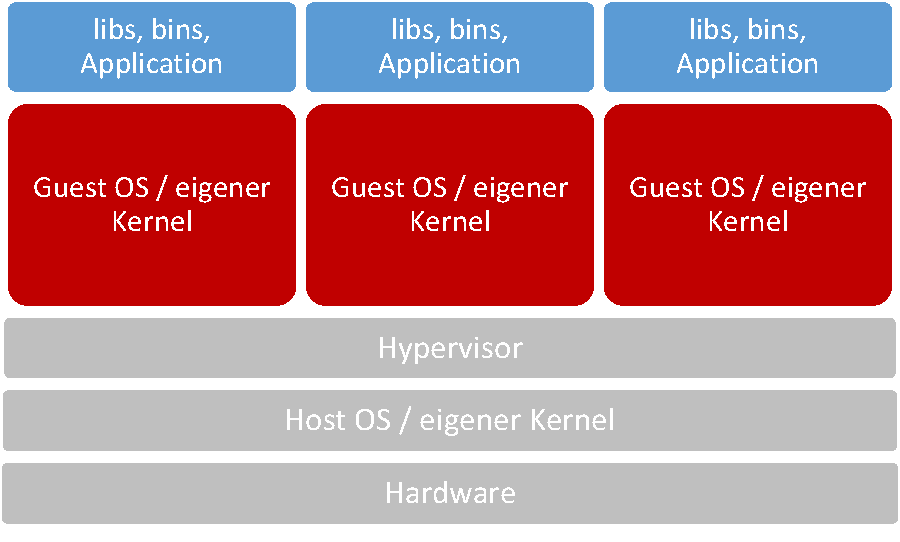
\includegraphics[width=0.49\textwidth]{bilder/vm-stack-virtualisation.pdf}}
		\caption{Container Isolation im Vergleich zu \glspl{acr-vm}}
		\label{fig:containerVsVm}
\end{figure}

Dieses Kapitel behandelt alle benötigten Grundlagen, die zur Isolation eines Prozesses benötigt werden. Es werden vorhandene Standards wie die \gls{acr-oci} und benötigte Systemcalls wie \gls{acr-chroot} näher erläutert. Zudem wird beschrieben, wie die Isolation, die Container bieten, durch Systemmittel des Linux\glspl{gls-kernel} selber erreicht werden kann.
\section{Standards}
\label{sec:standards}

\subsection{App Container}
\label{sec:appc}
\gls{acr-appc} ist ein Standard, der viele Aspekte innerhalb der Container-Landschaft behandelt. Dabei liegt die Hauptaufgabe darin, eine Laufzeitumgebung wie auch das \gls{gls-image}format und die Verbreitung von \glspl{gls-image} zu spezifizieren. Seit 2016 wird das Projekt nicht mehr aktiv weiterentwickelt. Bestandteile der \gls{acr-appc} wurden von der \gls{acr-oci} übernommen und dienen als Vorlage für die Spezifikation dieser.

\subsection{Open Container Initiative}
\label{sec:oci}
Die \gls{acr-oci} ist eine Initiative, die seit 2015 unter der Linux Foundation agiert. Das Ziel der OCI ist es, einen offenen Standard für Container zu schaffen, sodass die Wahl der Container-Laufzeitumgebung nicht mehr zu Inkompatibilität führt. Dabei liegt der Fokus auf eine einfache, schlanke Implementierung \citep{OpenContainerInitiative}.

Die OCI arbeitet aktuell an zwei Spezifikationen. Die runtime-spec standardisiert die Laufzeitumgebung  von Containern. Dabei wird festgelegt, welche Konfiguration, Prinzipien und Schnittstellen Laufzeitumgebungen stellen müssen. Um die Umsetzung der runtime-spec zu fördern, stellt die OCI eine beispielhafte Implementierung durch runC.

\begin{table}[h]
	\begin{center}
		\begin{tabular}{lcccc}
			\toprule
			& \multicolumn{2}{c}{Standard} & \multicolumn{2}{c}{Container Runtime}\\
			\cmidrule{2-5}
			& OCI		& appc		& Docker			& rkt					\\
			\midrule
			Container Image			& \faTimes	& \faCheck	& OCI image-spec 	& appc Image Format		\\
			Image Verbreitung		& \faTimes	& \faCheck	& Docker Registry	& appc Discovery Spec 	\\
			Lokales Speicherformat	& \faCheck	& \faTimes	& keine Spezifikation& keine Spezifikation	\\
			\midrule
			Runtime					& \faCheck	& \faCheck	& runC 				& appc runtime Spec		\\
			\bottomrule
		\end{tabular}
		\caption{Standards OCI und AppC im Vergleich \citep{MakingSenseofContainerStandardsandFoundations:OCICNCFAppcandRkt}}
		\label{tab:ociVSappc}
	\end{center}
\end{table}

Das zweite Projekt der OCI ist die image-spec. Dieses versucht einen Standard für \glspl{gls-image} zu definieren. Dabei plant die OCI nicht, vorhandene Image-Formate zu ersetzen, sondern auf diesen Aufzubauen und sie zu erweitern \citep{OpenContainerInitiative}.

Wie in \fref{tab:ociVSappc} zu sehen, wurden einige Konzepte des \gls{acr-appc}-Projekts in die \gls{acr-oci} übernommen. Vor allem die \gls{gls-image}-Spezifikation wurde durch die Mitarbeit ehemaliger \gls{acr-appc}-Maintainer gefördert. Allerdings sind einige Projekte noch nicht übernommen worden. So gibt es keine \gls{acr-oci} Spezifikation für die Verbreitung von \glspl{gls-image}, eines der meistgenutzten Features verschiedener Container-Runtimes. Um die Weiterentwicklung an solchen Projekten zu fördern wurden einige in die \gls{acr-cncf} übernommen \citep{MakingSenseofContainerStandardsandFoundations:OCICNCFAppcandRkt}.

\subsection{Cloud Native Computing Foundation}
\label{sec:cncf}
Die \gls{acr-cncf} beschäftigt sich im Gegensatz zur \gls{acr-oci} nicht nur mit Containern, sondern der kompletten \gls{gls-cloud}-Landschaft. Projekte wie \gls{acr-k8} und Prometheus werden durch die \gls{acr-cncf} weiterentwickelt und publiziert \citep{CloudNativeComputingFoundation}. Da der Cloud-Native Entwicklungsprozess von Containern getragen wird, spielen Technologien wie containerd und rkt eine entscheidende Rolle für die \gls{acr-cncf}.

\begin{figure}[h]
	\begin{center}
		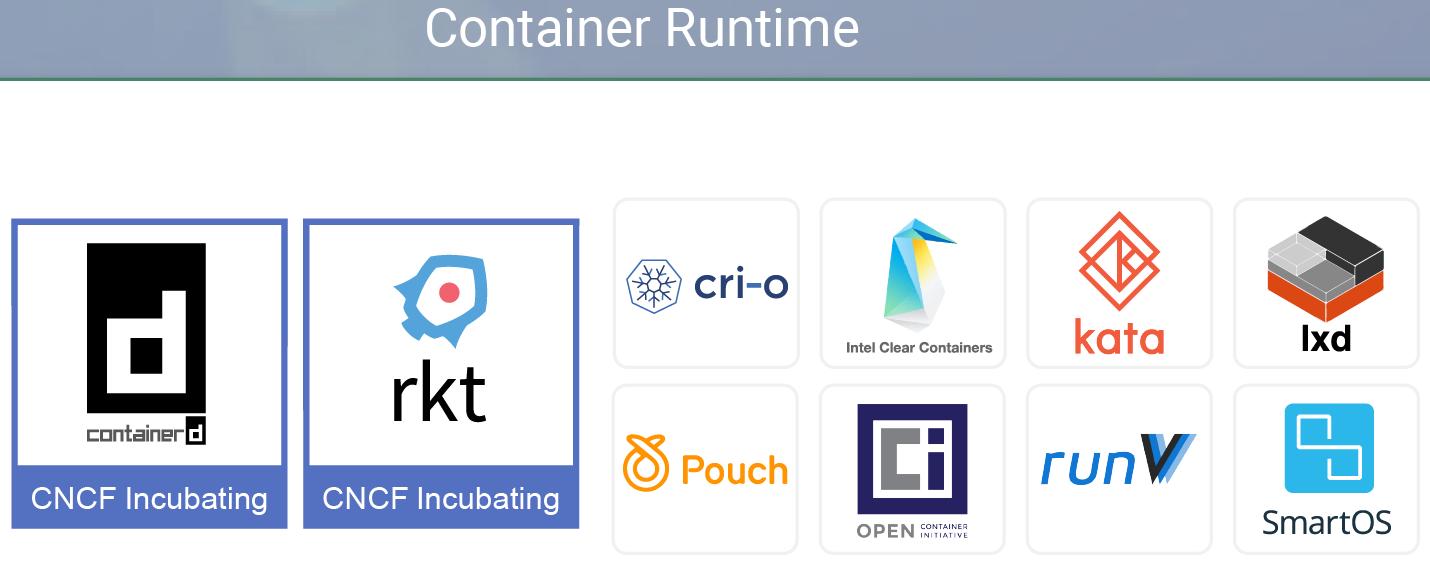
\includegraphics[scale=0.3]{bilder/cncf-container-landscape.png}
		\caption{CNCF Container Runtime Landschaft \citep{CNCFCloudNativeInteractiveLandscape}}
		\label{fig:cncfContainerLandscape}
	\end{center}
\end{figure}

Neben Container-Runtimes beinhaltet die \gls{acr-cncf} auch Projekte zur Orchestrierung wie \gls{acr-k8}, Logging und Monitoring wie auch Spezifikationen, zum Beispiel die TUF, eine Spezifikation die standardisiert, wie Softwarepakete upgedatet werden sollen \cite{CNCFCloudNativeInteractiveLandscape}. 

\section{Funktionsweise}
\label{sec:funktionsweise}

Container isolieren einzelne Prozesse durch verschiedene \gls{gls-kernel}-Technologien, die im Folgenden erklärt werden sollen.
\subsection{Change Root}
\label{sec:chroot}
\Gls{acr-chroot} ist ein Unix Systemaufruf, der es erlaubt einen Prozess in einem anderen Wurzelverzeichnis auszuführen \citep{Chroot1LinuxManualPage}. Daraus folgt, dass der Prozess in einer eigenen Verzeichnisstruktur arbeitet und keine Dateien des Host-\gls{acr-os} ändern kann. \Gls{acr-chroot} erlaubt somit die Isolierung des Dateisystems, die Container nutzen.

\subsection{Control Groups}
\label{sec:cgroups}
\glspl{acr-cgroup} dienen dazu, Systemressourcen für einzelne Prozesse zu limitieren. \todo{beschreibe cgroups, siehe \citep{ControlGroupV2}}

\subsection{Namespaces}
\label{sec:namespaces}

\subsection{Windows Hyper-V Container}
\label{sec:}

\todo{RunC Erklärung und ausführliche Beschreibung (libcontainer, runC, containerd ?, ...}

\section{Eigene Implementierung}
\label{sec:eigeneImpl}

Um die technischen Grundlagen zu vertiefen wurde eine eigene Container-Runtime entwickelt, die einen in Python geschriebenen Prozess isoliert und vom Hostsystem abschottet.